\newpage
\section{Greedy Algorithms}
别人恐惧我贪婪

\subsection{Activity Selection Problem}
Given a set of activities $S = \{ a_1, a_2, \dots, a_n \}$that wish to use a resource (e.g. a classroom).  Each $a_i$ takes place during a time interval $[s_i, f_i)$. Activities $a_i$ and $a_j$ are compatible if $f_j\le s_i$ or $f_i\le s_j$ (i.e. their time intervals do not overlap).

Select a maximum-size subset of mutually compatible activities.


\subsubsection{DP}
\begin{align*}
    c_{1,j}=\left\{ \begin{array}{ll}
        1 & \text{ if }j=1\\
        \max\{ c_{1,j-1},c_{1, k(j)} +1 \} & \text{ if }j>1
    \end{array} \right.
\end{align*}
where $c_{1,j}$ is the optimal solution for $a_1$ to $a_j$ , and $a_{k(j)}$ is the nearest compatible activity to $a_j$  that is finished before $a_j$ .

If each activity has a weight
\begin{align*}
    c_{1,j}=\left\{ \begin{array}{ll}
        w_j & \text{ if }j=1\\
        \max\{ c_{1,j-1},c_{1, k(j)} +w_j \} & \text{ if }j>1
    \end{array} \right.
\end{align*}
Greedy solution isn't correct with weighted activities. 

\subsubsection{Greedy}
Greedy Rule: Select the interval which ends first (but not overlapping the already chosen intervals). 

\begin{theorem}
    Consider any nonempty subproblem $S_k$, and let $a_m$ be an activity in $S_k$ with the earliest finish time.  Then $a_m$ is included in some maximum-size subset of mutually compatible activities of $S_k$. (用贪心策略得到的解元素代替最优解中的元素, 得到的解不会更差)
\end{theorem}

Implementation:
\begin{enumerate}
    \item Select the first activity; Recursively solve for the rest.
    \item Remove tail recursion by iterations.
\end{enumerate}
$O(N\log N)$

\subsection{Huffman Codes}
Representation of the original code in a binary tree. Find the full binary tree of minimum total cost where all characters are contained in the leaves.

\begin{lemma}
    Let $C$ be an alphabet in which each character $c \in C$ has frequency $c.freq$.  Let $x$ and $y$ be two characters in $C$ having the lowest frequencies.  Then there exists an optimal prefix code for $C$ in which the codewords for $x$ and $y$ have the same length and differ only in the last bit.
    \begin{figure}[!htb]
        \centering
        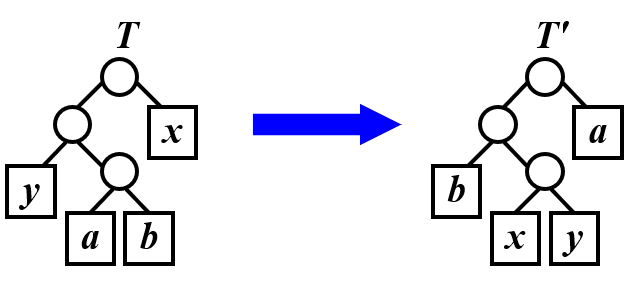
\includegraphics[width=0.309\textwidth]{pic/ADS9/Lemma1.png}
        % \caption{}
    \end{figure}
    \begin{align*}
        Cost(T)\ge Cost(T')
    \end{align*}
\end{lemma}

\begin{lemma}
    Let $C$ be a given alphabet with frequency $c.freq$ defined for each character $c \in C$.  Let $x$ and $y$ be two characters in $C$ with minimum frequency.  Let $C'$ be the alphabet $C$ with a new character $z$ replacing $x$ and $y$, and $z.freq = x.freq + y.freq$.  Let $T'$ be any tree representing an optimal prefix code for the alphabet $C'$.  Then the tree $T$, obtained from $T'$ by replacing the leaf node for $z$ with an internal node having $x$ and $y$ as children, represents an optimal prefix code for the alphabet $C$.
    \begin{figure}[!htb]
        \centering
        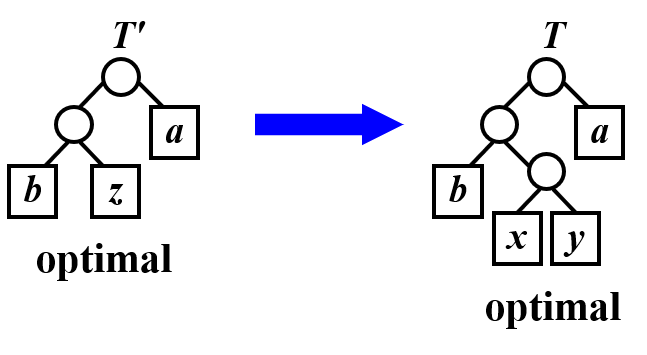
\includegraphics[width=0.309\textwidth]{pic/ADS9/Lemma2.png}
        % \caption{}
    \end{figure}
    \begin{align*}
        Cost(T')+x.freq+y.freq=Cost(T)
    \end{align*}
\end{lemma}
